\documentclass[a4paper, 11pt, oneside]{article}

\usepackage[utf8]{inputenc}
\usepackage[T1]{fontenc}
\usepackage[english]{babel}
\usepackage{fullpage}
\usepackage{enumerate}
\usepackage{enumitem}
\usepackage{graphicx}
\usepackage{url}
\usepackage{float}
\usepackage{titling}
\usepackage{listings}
\usepackage{hyperref,xcolor}
\renewcommand\maketitlehooka{\null\mbox{}\vfill}
\renewcommand\maketitlehookd{\vfill\null}

\hypersetup{
  colorlinks,
  allcolors=.,
  urlcolor=blue,
}

\newcommand{\ClassName}{INFO-0085: Compilers}
\newcommand{\ProjectName}{Implementing a VSOP compiler}
\newcommand{\AcademicYear}{2021 - 2022}

%%%% First page settings %%%%

\title{\ClassName\\\vspace*{0.8cm}\ProjectName\vspace{1cm}}
\author{Maxime Goffart \\180521 \and Olivier Joris\\182113}
\date{\vspace{1cm}Academic year \AcademicYear}

\begin{document}

%%% First page %%%

\begin{titlingpage}
{\let\newpage\relax\maketitle}
\end{titlingpage}

\newpage

%%%%%%%%%%%%%%%%%%%%%%%%%%%%%%%%%%%%%%%%%%

\section{Introduction}
\paragraph{}In this report, we provide a broad overview of our compiler implementation along with more detailed explanations on some parts of the implementation.

%%%%%%%%%%%%%%%%%%%%%%%%%%%%%%%%%%%%%%%%%%

\section{Tools}
\paragraph{}For some parts of the project, we have used external tools.

\paragraph{}For the lexical analysis part, we used Flex along with Bison. Specifically, Bison was used only to define the tokens used in Flex.\\
For the syntax analysis part, we continued to use Bison since we already used it for the lexical analysis part.\\
For the code generation part, we used the LLVM library. We have followed this \href{https://mukulrathi.com/create-your-own-programming-language/llvm-ir-cpp-api-tutorial/}{tutorial} to implement this last part. This choice
has been motivated by the fact that the library can optimize the generated code through its optimization passes.
%%%%%%%%%%%%%%%%%%%%%%%%%%%%%%%%%%%%%%%%%%

\section{Organization of the code} \label{codeOrg}
\paragraph{}Our code is split in multiple files. The files are the following:
\begin{itemize}
	\item \texttt{Makefile} is a Makefile to build the compiler by simply using the command \texttt{make}.
	\item \texttt{vsopc.l} is the file for the lexical analysis part using Flex.
	\item \texttt{vsopc.y} is the file for the syntax analysis part using Bison. It also contains the \texttt{main} function of the project.
	\item \texttt{*.cpp} and \texttt{*.hpp} are the implementation and header files for the possible tokens.
 	\item \texttt{runtime} is a folder containing the files necessary for the code generation part. It contains code for the external linkage with the object class and the power operation in respective \texttt{.c} and \texttt{.h} files.
\end{itemize}

\paragraph{}The classes defined in the \texttt{*.cpp} and \texttt{*.hpp} files are organized in an inheritance-based approach using dynamic dispatch because, in our opinion, it is the most natural approach while using an object-oriented language as C++. The hierarchy of classes can be represented by the figure \ref{classHierarchy}.
\begin{figure}
\centering
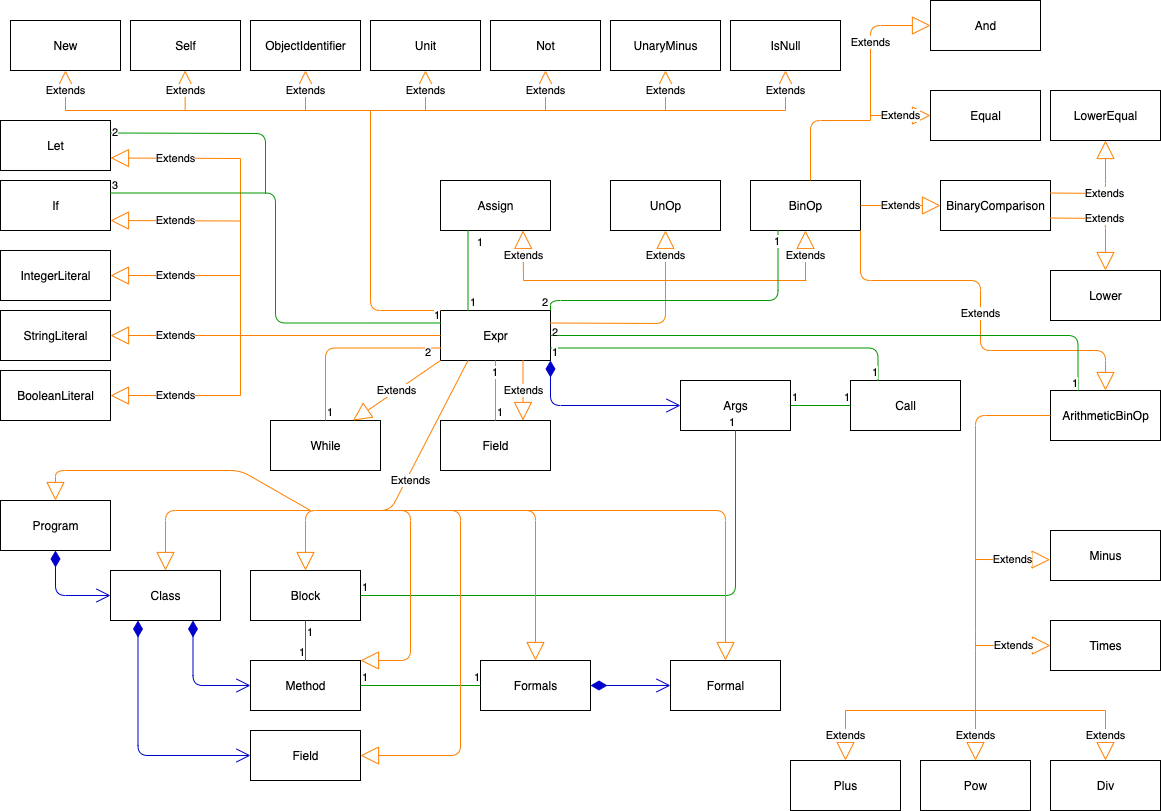
\includegraphics[scale=0.35]{uml.png}
\caption{Class hierarchy as a UML diagram}
\label{classHierarchy}
\end{figure}

%%%%%%%%%%%%%%%%%%%%%%%%%%%%%%%%%%%%%%%%%%

\section{Modules' responsibilities}
\paragraph{}Most \texttt{*.hpp} files contain the headers associated to at least one sub-type of expression. For instance, the file \texttt{while.hpp} contains the header associated to the \texttt{while} construct.\\
For each \texttt{.hpp} file, there is an associated \texttt{.cpp} file with the same name containing the implementation of the header.

\paragraph{}The \texttt{LLVM.cpp} file is a singleton responsible to make the link between our tokens and the LLVM library. 

\paragraph{}As already explained, \texttt{vsopc.l} contains the rules for the lexical analysis with Flex and \texttt{vsopc.y} contains the rules for the syntax analysis with Bison along with the \texttt{main} function.

%%%%%%%%%%%%%%%%%%%%%%%%%%%%%%%%%%%%%%%%%%

\section{Data structures and algorithms}
\paragraph{}Regarding data structures, we mostly use \texttt{std::vector}s defined in C++ standard template library (STL).

\paragraph{}For algorithms, we do not make use of algorithms that require any additional explanations than what is provided as documentation in the various source files.

%%%%%%%%%%%%%%%%%%%%%%%%%%%%%%%%%%%%%%%%%%

\section{Implementation choices}
\paragraph{}We decided to use Flex and Bison due to the strong recommendations made during the first presentation of the project.\\
Since we chose Flex and Bison, we were limited to C or C++ as programming languages. We decided to use C++ because we thought that having classes would come handy and, in our experience, it is easier to work with strings in C++ compared to C, even thought we have more experience in C than in C++.
Finally, as already mentioned in section \ref{codeOrg}, we decided to use an inheritance-based approach because, in our opinion, it is the most natural approach while using an OO language such as C++.

%%%%%%%%%%%%%%%%%%%%%%%%%%%%%%%%%%%%%%%%%%

\section{Conflicts in the grammar}
\paragraph{}Our grammar does not contain any shift/reduce or reduce/reduce conflicts.

%%%%%%%%%%%%%%%%%%%%%%%%%%%%%%%%%%%%%%%%%%

\section{Language extensions}
\paragraph{}Unfortunately, we did not have the time to implement any extension of the language.

%%%%%%%%%%%%%%%%%%%%%%%%%%%%%%%%%%%%%%%%%%

\section{Limitations, possible improvements, and retrospective}
\paragraph{}Our compiler support all the basic operations of the VSOP language and pass all tests of the submission platform. If we had more time, we would have implemented more features such as: a garbage collector, the support of decimals, some syntaxic sugar for instructions, etc.

\paragraph{}We did not regret the choice of C++ and the tools proposed by the professor and the assistant which saved us time. We just find it a pity that the LLVM library is poorly documented. Fortunately, the tutorial mentioned in the section 2 as well as the example code provided by the assistant have almost filled this gap. We also did not regret to use the inheritance-based approach using dynamic dispatch to implement our abstract syntax tree: we find
this approach very easily readable and understandable.
%%%%%%%%%%%%%%%%%%%%%%%%%%%%%%%%%%%%%%%%%%

\section{Time spent}
\paragraph{}Unfortunately, as we did not know that we would be asked the time spent at the end of the project, we did not keep track of it nor we can provide an approximation since we are always going back and forth between multiple projects specially with the integrated project.

%%%%%%%%%%%%%%%%%%%%%%%%%%%%%%%%%%%%%%%%%%
 
\end{document}
